\documentclass{ximera}

 

\usepackage{epsfig}

\graphicspath{
  {./}
  {figures/}
}

\usepackage{morewrites}
\makeatletter
\newcommand\subfile[1]{%
\renewcommand{\input}[1]{}%
\begingroup\skip@preamble\otherinput{#1}\endgroup\par\vspace{\topsep}
\let\input\otherinput}
\makeatother

\newcommand{\includeexercises}{\directlua{dofile("/home/jim/linearAlgebra/laode/exercises.lua")}}

%\newcounter{ccounter}
%\setcounter{ccounter}{1}
%\newcommand{\Chapter}[1]{\setcounter{chapter}{\arabic{ccounter}}\chapter{#1}\addtocounter{ccounter}{1}}

%\newcommand{\section}[1]{\section{#1}\setcounter{thm}{0}\setcounter{equation}{0}}

%\renewcommand{\theequation}{\arabic{chapter}.\arabic{section}.\arabic{equation}}
%\renewcommand{\thefigure}{\arabic{chapter}.\arabic{figure}}
%\renewcommand{\thetable}{\arabic{chapter}.\arabic{table}}

%\newcommand{\Sec}[2]{\section{#1}\markright{\arabic{ccounter}.\arabic{section}.#2}\setcounter{equation}{0}\setcounter{thm}{0}\setcounter{figure}{0}}

\newcommand{\Sec}[2]{\section{#1}}

\setcounter{secnumdepth}{2}
%\setcounter{secnumdepth}{1} 

%\newcounter{THM}
%\renewcommand{\theTHM}{\arabic{chapter}.\arabic{section}}

\newcommand{\trademark}{{R\!\!\!\!\!\bigcirc}}
%\newtheorem{exercise}{}

\newcommand{\dfield}{{\sf dfield9}}
\newcommand{\pplane}{{\sf pplane9}}

\newcommand{\EXER}{\section*{Exercises}}%\vspace*{0.2in}\hrule\small\setcounter{exercise}{0}}
\newcommand{\CEXER}{}%\vspace{0.08in}\begin{center}Computer Exercises\end{center}}
\newcommand{\TEXER}{} %\vspace{0.08in}\begin{center}Hand Exercises\end{center}}
\newcommand{\AEXER}{} %\vspace{0.08in}\begin{center}Hand Exercises\end{center}}

% BADBAD: \newcommand{\Bbb}{\bf}

\newcommand{\R}{\mbox{$\Bbb{R}$}}
\newcommand{\C}{\mbox{$\Bbb{C}$}}
\newcommand{\Z}{\mbox{$\Bbb{Z}$}}
\newcommand{\N}{\mbox{$\Bbb{N}$}}
\newcommand{\D}{\mbox{{\bf D}}}
\usepackage{amssymb}
%\newcommand{\qed}{\hfill\mbox{\raggedright$\square$} \vspace{1ex}}
%\newcommand{\proof}{\noindent {\bf Proof:} \hspace{0.1in}}

\newcommand{\setmin}{\;\mbox{--}\;}
\newcommand{\Matlab}{{M\small{AT\-LAB}} }
\newcommand{\Matlabp}{{M\small{AT\-LAB}}}
\newcommand{\computer}{\Matlab Instructions}
\newcommand{\half}{\mbox{$\frac{1}{2}$}}
\newcommand{\compose}{\raisebox{.15ex}{\mbox{{\scriptsize$\circ$}}}}
\newcommand{\AND}{\quad\mbox{and}\quad}
\newcommand{\vect}[2]{\left(\begin{array}{c} #1_1 \\ \vdots \\
 #1_{#2}\end{array}\right)}
\newcommand{\mattwo}[4]{\left(\begin{array}{rr} #1 & #2\\ #3
&#4\end{array}\right)}
\newcommand{\mattwoc}[4]{\left(\begin{array}{cc} #1 & #2\\ #3
&#4\end{array}\right)}
\newcommand{\vectwo}[2]{\left(\begin{array}{r} #1 \\ #2\end{array}\right)}
\newcommand{\vectwoc}[2]{\left(\begin{array}{c} #1 \\ #2\end{array}\right)}

\newcommand{\ignore}[1]{}


\newcommand{\inv}{^{-1}}
\newcommand{\CC}{{\cal C}}
\newcommand{\CCone}{\CC^1}
\newcommand{\Span}{{\rm span}}
\newcommand{\rank}{{\rm rank}}
\newcommand{\trace}{{\rm tr}}
\newcommand{\RE}{{\rm Re}}
\newcommand{\IM}{{\rm Im}}
\newcommand{\nulls}{{\rm null\;space}}

\newcommand{\dps}{\displaystyle}
\newcommand{\arraystart}{\renewcommand{\arraystretch}{1.8}}
\newcommand{\arrayfinish}{\renewcommand{\arraystretch}{1.2}}
\newcommand{\Start}[1]{\vspace{0.08in}\noindent {\bf Section~\ref{#1}}}
\newcommand{\exer}[1]{\noindent {\bf \ref{#1}}}
\newcommand{\ans}{}
\newcommand{\matthree}[9]{\left(\begin{array}{rrr} #1 & #2 & #3 \\ #4 & #5 & #6
\\ #7 & #8 & #9\end{array}\right)}
\newcommand{\cvectwo}[2]{\left(\begin{array}{c} #1 \\ #2\end{array}\right)}
\newcommand{\cmatthree}[9]{\left(\begin{array}{ccc} #1 & #2 & #3 \\ #4 & #5 &
#6 \\ #7 & #8 & #9\end{array}\right)}
\newcommand{\vecthree}[3]{\left(\begin{array}{r} #1 \\ #2 \\
#3\end{array}\right)}
\newcommand{\cvecthree}[3]{\left(\begin{array}{c} #1 \\ #2 \\
#3\end{array}\right)}
\newcommand{\cmattwo}[4]{\left(\begin{array}{cc} #1 & #2\\ #3
&#4\end{array}\right)}

\newcommand{\Matrix}[1]{\ensuremath{\left(\begin{array}{rrrrrrrrrrrrrrrrrr} #1 \end{array}\right)}}

\newcommand{\Matrixc}[1]{\ensuremath{\left(\begin{array}{cccccccccccc} #1 \end{array}\right)}}



\renewcommand{\labelenumi}{\theenumi)}
\newenvironment{enumeratea}%
{\begingroup
 \renewcommand{\theenumi}{\alph{enumi}}
 \renewcommand{\labelenumi}{(\theenumi)}
 \begin{enumerate}}
 {\end{enumerate}\endgroup}



\newcounter{help}
\renewcommand{\thehelp}{\thesection.\arabic{equation}}

%\newenvironment{equation*}%
%{\renewcommand\endequation{\eqno (\theequation)* $$}%
%   \begin{equation}}%
%   {\end{equation}\renewcommand\endequation{\eqno \@eqnnum
%$$\global\@ignoretrue}}

%\input{psfig.tex}

\author{Martin Golubitsky and Michael Dellnitz}

%\newenvironment{matlabEquation}%
%{\renewcommand\endequation{\eqno (\theequation*) $$}%
%   \begin{equation}}%
%   {\end{equation}\renewcommand\endequation{\eqno \@eqnnum
% $$\global\@ignoretrue}}

\newcommand{\soln}{\textbf{Solution:} }
\newcommand{\exercap}[1]{\centerline{Figure~\ref{#1}}}
\newcommand{\exercaptwo}[1]{\centerline{Figure~\ref{#1}a\hspace{2.1in}
Figure~\ref{#1}b}}
\newcommand{\exercapthree}[1]{\centerline{Figure~\ref{#1}a\hspace{1.2in}
Figure~\ref{#1}b\hspace{1.2in}Figure~\ref{#1}c}}
\newcommand{\para}{\hspace{0.4in}}

\renewenvironment{solution}{\suppress}{\endsuppress}

\ifxake
\newenvironment{matlabEquation}{\begin{equation}}{\end{equation}}
\else
\newenvironment{matlabEquation}%
{\let\oldtheequation\theequation\renewcommand{\theequation}{\oldtheequation*}\begin{equation}}%
  {\end{equation}\let\theequation\oldtheequation}
\fi

\makeatother


\title{The Initial Value Problem and Eigenvectors}

\begin{document}
\begin{abstract}
\end{abstract}
\maketitle


\label{S:IVP&E} \index{initial value problem}

The general {\em constant coefficient\/}
\index{system of differential equations!constant coefficient}
system of differential equations has the form
\renewcommand{\arraystretch}{1.8}
\begin{equation}\label{lingen}
\begin{array}{ccc}
\dps \frac{dx_1}{dt}(t) & = & c_{11}x_1(t) + \cdots + c_{1n}x_n(t) \\
\vdots  & \vdots & \vdots \\
\dps \frac{dx_n}{dt}(t) & = & c_{n1}x_1(t) + \cdots + c_{nn}x_n(t)
\end{array}
\end{equation}
\renewcommand{\arraystretch}{1.0}%
where the coefficients $c_{ij}\in \R$ are constants.  Suppose that 
\eqref{lingen} satisfies the initial conditions $x_1(0) = K_1$, \ldots,  
$x_n(0) = K_n$.

Using matrix multiplication of a vector and matrix, we can rewrite these 
differential equations in a compact form.   Consider the $n\times n$ 
coefficient matrix
\[
C = \left(
\begin{array}{rrrr}
 c_{11} & c_{12} & \cdots & c_{1n} \\
 c_{21} & c_{22} & \cdots & c_{2n}  \\
 \vdots & \vdots &        & \vdots  \\
 c_{n1} & c_{n2} & \cdots & c_{nn}
\end{array}
\right)
\]
and the $n$ vectors of initial conditions and unknowns
\[
X_0=\left(
\begin{array}{ccc}
K_1 \\ \vdots  \\ K_n
\end{array}
\right) \AND
X=\left(
\begin{array}{ccc}
x_1 \\ \vdots  \\ x_n
\end{array}
\right).
\]
Then \eqref{lingen} has the compact form
\begin{equation}  \label{E:geneqn}
\begin{array}{rcl}
\dps\frac{dX}{dt} & = & CX\\
X(0) & = & X_0.  
\end{array}
\end{equation}


In Section~\ref{s:3.5}, we plotted the phase space picture 
of the planar system of differential equations
\begin{equation} \label{-13}
\vectwo{\dot{x}}{\dot{y}}
= C \vectwo{x(t)}{y(t)}
\end{equation}
where
\[
C = \mattwo{-1}{3}{3}{-1}.
\]
In those calculations we observed that there is a solution to
\eqref{-13} that stayed on the main diagonal for each moment in
time.  Note that a vector is on the main diagonal if it is a
scalar multiple of $\vectwo{1}{1}$.  Thus a solution that stays
on the main diagonal for all time $t$ must have the form
\begin{equation} \label{e:diagform}
\vectwo{x(t)}{y(t)} = u(t) \vectwo{1}{1}
\end{equation}
for some real-valued function $u(t)$.  When a function of form
\eqref{e:diagform} is a solution to \eqref{-13}, it satisfies:
\begin{align*}
  \dot{u}(t)\vectwo{1}{1} &= \vectwo{\dot{x}(t)}{\dot{y}(t)} 
                            = C \vectwo{x(t)}{y(t)} \\
                          &= C u(t)\vectwo{1}{1} = u(t) C \vectwo{1}{1}.
\end{align*}
A calculation shows that
\[
C \vectwo{1}{1} = 2 \vectwo{1}{1}.
\]
Hence
\[
\dot{u}(t) \vectwo{1}{1} =  2 u(t) \vectwo{1}{1}.
\]
It follows that the function $u(t)$ must satisfy the
differential equation
\[
\frac{du}{dt} = 2u.
\]
whose solutions are
\[
u(t) = \alpha e^{2t},
\]
for some scalar $\alpha$.

Similarly, we also saw in our \Matlab experiments that there was
a solution that for all time stayed on the anti-diagonal, the
line $y=-x$.  Such a solution must have the form
\[
\vectwo{x(t)}{y(t)} = v(t) \vectwo{1}{-1}.
\]
A similar calculation shows that $v(t)$ must satisfy the
differential equation
\[
\frac{dv}{dt} = -4v.
\]
Solutions to this equation all have the form
\[
v(t) = \beta e^{-4t},
\]
for some real constant $\beta$.

Thus, using matrix multiplication, we are able to prove
analytically that there are solutions to \eqref{-13} of exactly
the type suggested by our \Matlab experiments.  However, even
more is true and this extension is based on the principle of 
superposition that was introduced for algebraic equations in 
Section~\ref{S:Superposition}.  

\subsection*{Superposition in Linear Differential Equations}
\index{superposition}\index{differential equation!superposition}

Consider a general linear differential equation of the form
\begin{equation} \label{gen1}
\frac{dX}{dt} = CX,
\end{equation}
where $C$ is an $n\times n$ matrix.  Suppose that $Y(t)$ and
$Z(t)$ are solutions to \eqref{gen1} and $\alpha,\beta\in\R$ are
scalars.  Then $X(t)=\alpha Y(t)+\beta Z(t)$ is also a solution.
We verify this fact using the `linearity' of $d/dt$.  Calculate
\begin{eqnarray*}
\frac{d}{dt} X(t) & = &
\alpha \frac{dY}{dt}(t) + \beta \frac{dZ}{dt}(t) \\
 & = &\alpha CY(t) + \beta CZ(t)\\
 & = & C(\alpha Y(t) + \beta Z(t))\\
 & = & CX(t).
\end{eqnarray*}
So superposition is valid for solutions of linear differential equations.


\subsection*{Initial Value Problems}
\index{initial value problem}

Suppose that we wish to find a solution to
\eqref{-13} satisfying the initial conditions\index{initial condition}
\[
\left(\begin{array}{c} x(0) \\ y(0) \end{array}\right) =
\left(\begin{array}{c}1\\3\end{array}\right).
\]
Then we can use the principle of superposition to find this solution in 
closed form.  Superposition implies that for each pair of scalars 
$\alpha,\beta\in\R$, the functions
\begin{equation}  \label{e:solnODE}
\left(\begin{array}{c} x(t) \\ y(t) \end{array}\right) =
\alpha e^{2t}\left(\begin{array}{c}1\\1\end{array}\right) +
\beta e^{-4t}\left(\begin{array}{r} 1\\-1\end{array}\right),
\end{equation}
are solutions to \eqref{-13}.  Moreover, for a solution of this form 
\[
\left(\begin{array}{c} x(0) \\ y(0) \end{array}\right) =
\left(\begin{array}{c} \alpha+\beta \\ \alpha-\beta
\end{array}\right).
\]

Thus we can solve our prescribed initial value problem, if we can
solve the system of linear equations
\begin{eqnarray*}
\alpha + \beta = 1\ \\
\alpha - \beta = 3.
\end{eqnarray*}
This system is solved for $\alpha=2$ and $\beta=-1$. Thus
\[
\vectwo{x(t)}{y(t)} = 2e^{2t}\vectwo{1}{1} - e^{-4t}\vectwo{1}{-1}
\]
is the desired closed form solution.

\subsection*{Eigenvectors and Eigenvalues}

We emphasize that just knowing that there are two lines in the
plane that are invariant under the dynamics of the system of
linear differential equations is sufficient information to solve
these equations.  So it seems appropriate to ask the question:
When is there a line that is invariant under the dynamics of a
system of linear differential equations?  This question is
equivalent to asking:  When is there a nonzero vector $v$ and a
nonzero real-valued function $u(t)$ such that
\[
X(t) = u(t) v
\]
is a solution to \eqref{gen1}?

Suppose that $X(t)$ is a solution to the system of differential
equations $\dot{X}=CX$.  Then $u(t)$ and $v$ must satisfy
\begin{equation}  \label{E:diffdir}
\dot{u}(t)v = \frac{dX}{dt} = CX(t) = u(t) Cv.
\end{equation}
Since $u$ is nonzero, it follows that $v$ and $Cv$ must lie on the
same line through the origin.  Hence
\begin{equation}  \label{e:eigendef}
Cv = \lambda v,
\end{equation}
for some real number $\lambda$.

\begin{definition}  \label{D:eigenvalue1}
A nonzero vector $v$ satisfying \eqref{e:eigendef} is called an
{\em eigenvector\/} \index{eigenvector} of the matrix $C$, and
the number $\lambda$ is an {\em eigenvalue\/} \index{eigenvalue}
of the matrix $C$.
\end{definition}
Geometrically, the matrix $C$ maps an eigenvector onto a multiple
of itself --- that multiple is the eigenvalue.

Note that scalar multiples of eigenvectors are also eigenvectors.  More 
precisely:
\begin{lemma}  \label{L:e'vector}
Let $v$ be an eigenvector of the matrix $C$ with eigenvalue $\lambda$.   
Then $\alpha v$ is also an eigenvector of $C$ with eigenvalue $\lambda$ 
as long as $\alpha\neq 0$.
\end{lemma}

\begin{proof} By assumption, $Cv=\lambda v$ and $v$ is nonzero. Now calculate
\[
C(\alpha v) = \alpha Cv = \alpha\lambda v = \lambda(\alpha v).
\]
The lemma follows from the definition of eigenvector.  \end{proof}

It follows from \eqref{E:diffdir} and \eqref{e:eigendef} that if $v$ is
an eigenvector of $C$ with eigenvalue $\lambda$, then
\[
\frac{du}{dt} = \lambda u.
\]
Thus we have returned to our original linear differential
equation that has solutions
\[
u(t) = Ke^{\lambda t},
\]
for all constants $K$.

We have proved the following theorem.
\begin{theorem}  \label{T:eigensoln}
Let $v$ be an eigenvector of the $n\times n$ matrix $C$ with
eigenvalue $\lambda$.  Then
\[
X(t) = e^{\lambda t}v
\]
is a solution to the system of differential equations $\dot{X}=CX$.
\end{theorem}



Finding eigenvalues and eigenvectors from first principles --- even for 
$2\times 2$ matrices --- is not a simple task.  We end this section with 
a calculation illustrating that real eigenvalues need not exist.  In 
Section~\ref{S:evchp}, we present a natural method for computing  
eigenvalues (and eigenvectors) of $2\times2$ matrices.  We defer the 
discuss of how to find eigenvalues and eigenvectors of $n\times n$ matrices 
until Chapter~\ref{C:D&E}.


\subsubsection*{An Example of a Matrix with No Real Eigenvalues}

Not every matrix has {\em real\/} eigenvalues\index{eigenvalue!real} and
eigenvectors\index{eigenvector!real}.  Recall the linear system of differential 
equations $\dot{x}=Cx$ whose phase plane is pictured in Figure~\ref{pp_dsp2}.  
That phase plane showed no evidence of an invariant line and indeed there is 
none.  The matrix $C$ in that example was
\[
C=\mattwo{-1}{-2}{3}{-1}.
\]
We ask: Is there a value of $\lambda$ and a nonzero vector
$(x,y)$ such that
\begin{equation}  \label{E:eigexamp}
C\left(\begin{array}{c} x\\y\end{array}\right) =
\lambda  \left(\begin{array}{c} x\\y\end{array}\right)?
\end{equation}
Equation \eqref{E:eigexamp} implies that
\[
\left(\begin{array}{cc} -1-\lambda & -2 \\ 3 & -1-\lambda
\end{array}\right) \left(\begin{array}{c}
x\\y\end{array}\right) =0.
\]
If this matrix is row equivalent to the identity matrix, then
the only solution of the linear system is $x=y=0$.  To have a
nonzero solution, the matrix
\[
\left(\begin{array}{cc} -1-\lambda & -2 \\ 3 & -1-\lambda
\end{array}\right)
\]
must not be row equivalent to $I_2$.  Dividing the $1^{st}$ row by
$-(1+\lambda)$ leads to
\[
\left(\begin{array}{cc} 1 & \frac{2}{1+\lambda} \\ 3 & -1-\lambda
\end{array}\right).
\]
Subtracting $3$ times the $1^{st}$ row from the second produces
the matrix
\[
\left(\begin{array}{cc} 1 & \frac{2}{1+\lambda} \\ 0 &
-(1+\lambda) - \frac{6}{1+\lambda}
\end{array}\right).
\]
This matrix is not row equivalent to $I_2$ when the lower
right hand entry is zero; that is, when
\[
(1+\lambda) +\frac{6}{1+\lambda} = 0.
\]
That is, when
\[
(1+\lambda)^2 = -6,
\]
which is not possible for any real number $\lambda$.  This
example shows that the question of whether a given matrix has a
real eigenvalue and a real eigenvector --- and hence when the
associated system of differential equations has a line that is
invariant under the dynamics --- is a subtle question.

Questions concerning eigenvectors and eigenvalues are central to
much of the theory of linear algebra.  We discuss this
topic for $2\times 2$ matrices in Section~\ref{S:evchp} and
Chapter~\ref{Chap:Planar} and for general square matrices in
Chapters~\ref{C:D&E} and \ref{C:HDeigenvalues}.

\EXER

\TEXER

\begin{exercise} \label{c4.1.5}
Write the system of linear ordinary differential equations
\begin{eqnarray*}
\frac{dx_1}{dt}(t) & = & 4x_1(t) + 5x_2(t) \\
\frac{dx_2}{dt}(t) & = & 2x_1(t) - 3x_2(t)
\end{eqnarray*}
in matrix form.

\begin{solution}
\ans
\arraystart
\[
\left(\begin{array}{r} \dps\frac{dx_1}{dt}(t) \\ 
\dps\frac{dx_2}{dt}(t)\end{array}\right) =
\left(\begin{array}{rr} 4 & 5 \\ 2 & -3\end{array}\right)
\left(\begin{array}{r} x_1(t) \\ x_2(t)\end{array}\right)
\]
\arrayfinish

\end{solution}
\end{exercise}

\begin{exercise} \label{c4.4.4}
Show that all solutions to the system of linear differential equations
\begin{eqnarray*}
\frac{dx}{dt} & = & 3x \\
\frac{dy}{dt} & = & -2y
\end{eqnarray*}
are linear combinations of the two solutions
\[
U(t) = e^{3t}\vectwo{1}{0} \AND V(t) = e^{-2t}\vectwo{0}{1}.
\]

\begin{solution}

The system is uncoupled, so we can solve each equation
independently, using the initial value problem to obtain:
\[ \begin{array}{rcl}
x(t) & = & x_0e^{3t} \\
y(t) & = & y_0e^{-2t}. \end{array} \]
All solutions are of the form
\[ \vectwo{x(t)}{y(t)} = \vectwo{x_0e^{3t}}{y_0e^{-2t}}
= x_0\left(e^{3t}\vectwo{1}{0}\right) +
y_0\left(e^{-2t}\vectwo{0}{1}\right). \]
So all solutions are linear combinations of
\[ 
U(t) = e^{3t}\vectwo{1}{0} \AND V(t) = e^{-2t}\vectwo{0}{1}. 
\]

\end{solution}
\end{exercise}

\begin{exercise} \label{c4.5.1}
Consider
\begin{equation}  \label{e:Ceqn}
\frac{dX}{dt}(t) = CX(t)
\end{equation}
where
\[
C=\left(\begin{array}{cr} 2 & 3\\0& -1 \end{array}\right).
\]
Let
\[
v_1=\left(\begin{array}{c} 1\\0\end{array}\right)\AND
v_2=\left(\begin{array}{r} 1\\-1\end{array}\right),
\]
and let
\[
Y(t)=e^{2t} v_1 \AND Z(t)=e^{-t}v_2.
\]
\begin{enumeratea}
\item Show that $Y(t)$ and $Z(t)$ are solutions to \eqref{e:Ceqn}.
\item Show that $X(t)=2Y(t)-14Z(t)$ is a solution to \eqref{e:Ceqn}.
\item Use the principle of superposition to verify that
$X(t)=\alpha Y(t) + \beta Z(t)$ is a solution to \eqref{e:Ceqn}.
\item Using the general solution found in part (c), find a solution
$X(t)$ to \eqref{e:Ceqn} such that
\[
X(0) = \left(\begin{array}{r} 3\\-1\end{array}\right).
\]
\end{enumeratea}

\begin{solution}
\soln
\begin{enumeratea}
\item In order to determine that $Y(t)$ is a solution
to \eqref{e:Ceqn}, substitute $Y(t)$ into both sides of the 
equation $\frac{dX}{dt} = CX$:
\[
\frac{dY}{dt}
= \frac{d}{dt}\left(e^{2t}\vectwo{1}{0}\right)
= \frac{d}{dt}\cvectwo{e^{2t}}{0}
= \cvectwo{2e^{2t}}{0};
\]
\[
CY(t)
= \mattwo{2}{3}{0}{-1}\cvectwo{e^{2t}}{0}
= \cvectwo{2e^{2t}}{0}.
\]
Similarly, show that $Z(t)$ is a solution:
\[
\frac{dZ}{dt}
= \frac{d}{dt}\left(e^{-t}\vectwo{1}{-1}\right)
= \frac{d}{dt}\cvectwo{e^{-t}}{-e^{-t}}
= \cvectwo{-e^{-t}}{e^{-t}};
\]
\[
CZ(t)
= \mattwo{2}{3}{0}{-1}\cvectwo{e^{-t}}{-e^{-t}}
= \cvectwo{-e^{-t}}{e^{-t}}.
\]

\item Again, verify that $X(t) = 2Y(t) - 14Z(t)$ is a solution to
\eqref{e:Ceqn} by substituting into both sides of the equation and
noting that the values are equal:
\[
\frac{dX}{dt}
= \frac{d}{dt}\left(2e^{2t}\vectwo{1}{0} - 14e^{-t}\vectwo{1}{-1}\right)
= \frac{d}{dt}\cvectwo{2e^{2t} - 14e^{-t}}{14e^{-t}} 
= \cvectwo{4e^{2t} + 14e^{-t}}{-14e^{-t}};
\]
\[
CX(t) = C\left(2Y(t) - 14Z(t)\right)
= C\left(\cvectwo{2e^{2t}}{0} - \cvectwo{14e^{-t}}{-14e^{-t}}\right)
= \cvectwo{4e^{2t} + 14e^{-t}}{-14e^{-t}}.
\]

\item As demonstrated in Section~\ref{S:Superposition}, if
$Y(t)$ and $Z(t)$ are both solutions to
\eqref{e:Ceqn}, then $X(t) = \alpha Y(t) + \beta Z(t)$ is also
a solution to \eqref{e:Ceqn}.

\item  \ans 
\[
X(t) = 2e^{2t}\vectwo{1}{0} + e^{-t}\vectwo{1}{-1}.
\]

\soln Note that
\[ X(t) = \alpha Y(t) + \beta Z(t) = \alpha e^{2t}\vectwo{1}{0}
+ \beta e^{-t}\vectwo{1}{-1} \]
is a solution to \eqref{e:Ceqn}.  Substitute the value
$X(0) = (3,-1)^t$  into the equation to find a solution with that
initial condition:
\[
\vectwo{3}{-1} = X(0) = \alpha\vectwo{1}{0} +
\beta\vectwo{1}{-1}.
\]
We now have the linear system:
\[ \begin{array}{rrrrr}
3 & = & \alpha & + & \beta \\
-1 & = & & & -\beta \end{array} \]
which we can solve to find $\alpha = 2$ and $\beta = 1$.
\end{enumeratea}

\end{solution}
\end{exercise}

\begin{exercise} \label{c4.5.2}
Find a solution to
\[
\dot{X}(t)=CX(t)
\]
where
\[
C=\mattwo{1}{-1}{-1}{1}
\]
and
\[
X(0)=\vectwo{2}{1}.
\]
{\bf Hint:} Observe that
\[
\vectwo{1}{1} \AND \vectwo{1}{-1}
\]
are eigenvectors of $C$.

\begin{solution}

\ans 
\[
X(t) = \frac{3}{2}\vectwo{1}{1} + \frac{1}{2}e^{2t}\vectwo{1}{-1}.
\]

\soln Note that if $Cv = \lambda v$, then $X(t) = e^{\lambda t}v$ is a
solution to $\dot{X}(t) = CX(t)$.  Let
\[
v_1 = \vectwo{1}{1} \AND v_2 = \vectwo{1}{-1}.
\]
The eigenvalues corresponding to $v_1$ and $v_2$ are
$\lambda_1 = 0$ and $\lambda_2 = 2$.  This can be verified
by calculating $Cv_1 = 0$ and $Cv_2 = 2v_2$.
So,
\[
X(t) = \vectwo{1}{1} \AND X(t) = e^{2t}\vectwo{1}{-1}
\]
are both solutions to $\dot{X}(t) = CX$.  By the principle of
superposition,
\[
X(t) = \alpha\vectwo{1}{1} + \beta e^{2t}\vectwo{1}{-1}
\]
is also a solution.
Substitute the given the initial condition into the equation to obtain
\[
\vectwo{2}{1} = X(0) = \alpha\vectwo{1}{1} + \beta\vectwo{1}{-1}.
\]
Now, solve the linear system
\[
\begin{array}{rrrrr}
2 & = & \alpha & + & \beta \\
1 & = & \alpha & - & \beta \end{array}
\]
to find that $\alpha = \frac{3}{2}$ and $\beta = \frac{1}{2}$.


\end{solution}
\end{exercise}

\begin{exercise} \label{c4.5.3}
Let
\[
C=\mattwo{a}{b}{b}{a}.
\]
Show that
\[
\vectwo{1}{1} \AND \vectwo{1}{-1}
\]
are eigenvectors of $C$.  What are the corresponding eigenvalues?

\begin{solution}

\ans Let
\[ v_1 = \vectwo{1}{1} \AND v_2 = \vectwo{1}{-1}. \]
The vector $v_1$ is an eigenvector of $C$ with corresponding
eigenvalue $a + b$, and $v_2$ is an eigenvector with eigenvalue $a - b$.

\soln Calculate
\[ Cv_1 = \mattwo{a}{b}{b}{a}\vectwo{1}{1} = \vectwo{a + b}{a + b} =
(a + b)\vectwo{1}{1}. \]
\[ Cv_2 = \mattwo{a}{b}{b}{a}\vectwo{1}{-1} = \vectwo{a - b}{b - a} =
(a - b)\vectwo{1}{-1}. \]


\end{solution}
\end{exercise}

\begin{exercise} \label{c4.5.4}
Let
\[
C=\mattwo{1}{2}{-3}{-1}.
\]
Show that $C$ has no real eigenvectors.

\begin{solution}

A vector $(x,y)$ is an eigenvector of $C$ if
\[ C\vectwo{x}{y} = \lambda\vectwo{x}{y} \]
that is, if
\[ (C - \lambda I_2)\vectwo{x}{y} = 0. \]
In this case,
\[ \cmattwo{1 - \lambda}{2}{-3}{-1 - \lambda}
\vectwo{x}{y} = 0. \]
This equation will have a nonzero solution $(x,y)$ only if
\[ \cmattwo{1 - \lambda}{2}{-3}{-1 - \lambda}\vectwo{x}{y} \]
is not row equivalent to the identity matrix.
Row reducing the matrix yields
\[ \cmattwo{1}{\frac{2}{1 - \lambda}}{0}
{-1 - \lambda + \frac{6}{1-\lambda}} \]
so $C$ has an eigenvector when
\[ -1 - \lambda + \frac{6}{1-\lambda} = 0, \]
that is, when $\lambda^2 = -5$.  Therefore, $C$ has no real 
eigenvectors.

\end{solution}
\end{exercise}

\begin{exercise}  \label{c4.9.6A}
Suppose that $A$ is an $n\times n$ matrix with zero as an eigenvalue.
Show that $A$ is not invertible.  {\bf Hint:}  Assume that $A$ is invertible 
and compute $A\inv Av$ where $v$ is an eigenvector of $A$ corresponding to 
the zero eigenvalue.

\begin{solution}
\soln
Suppose that $A$ is an $n\times n$ matrix with zero eigenvalue.  We need to
prove that $A$ is not invertible.  Let $v\in\R^n$ be a nonzero 
eigenvector corresponding to the zero eigenvalue.  Therefore, $Av=0$. 
Suppose that $A\inv$ exists.  Then
\[
v = I_nv = A\inv Av = A\inv 0 = 0,
\]
which is a contradiction.  Therefore, $A$ is not invertible.

\end{solution}
\end{exercise}
\noindent {\bf Remark:}  In fact, $A$ is invertible\index{invertible} if 
all of the eigenvalues of $A$ are nonzero.  See Corollary~\ref{C:eig=0} of 
Chapter~\ref{C:D&E}.


\CEXER

\begin{exercise} \label{c4.5.6}
Consider the matrix $A$ and vector $X_0$ given by
\[
A=\mattwo{2}{1}{0}{1}\AND X_0=\vectwo{1}{1}.
\]
Use {\sf map} to compute $X_1 = AX_0$, $X_2 = AX_1$, $X_3=AX_2$ etc.\ by a
repeated use of the {\sf Map} button in the {\sf MAP Display} window.  What
do you observe?  What happens if you start the iteration process with a
different choice for $X_0$, and, in particular, for an $X_0$ that is close
to $\vectwo{-1}{1}$?

\begin{solution}

For each iteration, the $y$-coordinate of the solution is $1$.  After a
number of iterations, the $x$-coordinate approaches infinity, so the
direction of the solution vector approaches $(1,0)$, which, as shown
in Exercise~\ref{c4.5.5a}, is an eigenvector of $A$.  For any $X_0
\neq (-1,1)$, the solution vector approaches the direction
$(1,0)$.  If $X_0 = (-1,1)$ or some multiple thereof, then the solution
vectors remains on the line $y = -x$, since $(-1,1)$ is also an
eigenvector of $A$.

\end{solution}
\end{exercise}

\noindent In Exercises~\ref{c4.5.5a} -- \ref{c4.5.5b} use {\sf map} to find
an (approximate) eigenvector for the given matrix.  {\bf Hint:} Choose a
vector in {\sf map} and repeatedly click on the button {\sf Map} until the
vector maps to a multiple of itself.  You may wish to use the {\sf Rescale} 
feature in the {\sf MAP Options}.  Then the length of the vector is rescaled 
to one after each use of the command {\sf Map}. In this way, you can avoid
overflows in the computations while still being able to see the
directions where the vectors are moved by the matrix mapping.  The coordinates 
of the new vector obtained by applying {\sf map} can be viewed in the 
{\sf Vector input} window.

\begin{exercise} \label{c4.5.5a}
$B=\mattwo{2}{-2}{2}{7}$.

\begin{solution}
The vector $(-1,2)^t$ is an eigenvector of $B$ with
corresponding eigenvalue $6$, and $(-2,1)^t$ is an eigenvector with
corresponding eigenvalue $3$.


\end{solution}
\end{exercise}
\begin{exercise} \label{c4.5.5b}
$C=\mattwo{1}{1.5}{0}{-2}$.

\begin{solution}
The vector $(-1,2)^t$ is an eigenvector of $C$ with
corresponding eigenvalue $-2$, and the vector $(1,0)^t$ is an eigenvector
with eigenvalue $1$.


\end{solution}
\end{exercise}

\begin{exercise} \label{c4.4.5}
Use \Matlab to verify that solutions to the system of linear differential
equations
\begin{eqnarray*}
\frac{dx}{dt} & = & 2x + y\\
\frac{dy}{dt} & = & y
\end{eqnarray*}
are linear combinations of the two solutions
\[
U(t) = e^{2t}\vectwo{1}{0} \AND V(t) = e^{t}\vectwo{-1}{1}.
\]
More concretely, proceed as follows:
\begin{itemize}
\item[(a)]  By superposition, the general solution to the differential
equation has the form $X(t)=\alpha U(t) + \beta V(t)$.  Find constants
$\alpha$ and $\beta$ such that $\alpha U(0) + \beta V(0) = \vectwo{0}{1}$.
\item[(b)] Graph the second component $y(t)$ of this solution using the
\Matlab {\tt plot} command.
\item[(c)] Use {\pplane} to compute a solution via the {\sf Keyboard
input} starting at $(x(0),y(0)) = (0,1)$ and then use the
{\tt y} {\tt vs} {\tt t} command in {\pplane} to graph this solution.
\item[(d)] Compare the results of the two plots.
\item[(e)]  Repeat steps (a)--(d) using the initial vector $\vectwo{1}{1}$.
\end{itemize}

\begin{solution}

(a) \ans If $\alpha = 1$ and $\beta = 1$, then
\[
\alpha U(0) + \beta V(0) = \vectwo{0}{1}. 
\]

\soln Solve the linear system
\[
\begin{array}{rrrrl}
\alpha & - & \beta & = & 0 \\
& & \beta & = & 1. \end{array}
\]

(b) Figure~\ref{c4.4.5}a shows $y$ as a function of $t$.  The figure
was created by the \Matlab commands:
\begin{verbatim}
t = linspace(-8,2);
y = exp(t);
plot(t,y)
\end{verbatim}

(c) Figure~\ref{c4.4.5}b shows the {\tt pplane5} graph of the system,
and Figure~\ref{c4.4.5}c shows the {\tt y vs.\ t} graph.

(d) The two plots are identical, since the {\tt pplane5} command
{\tt y vs.\ t} graphs the $y$ component of the solution, which is
precisely what we did by hand in (b).

(e) In this case, $\alpha = 2$ and $\beta = 1$.  Since the $y$
component of $U(t)$ is zero, the graphs of $y(t)$ are identical
to those in (b) and (c).

\begin{figure}[htb]
                       \centerline{%
                       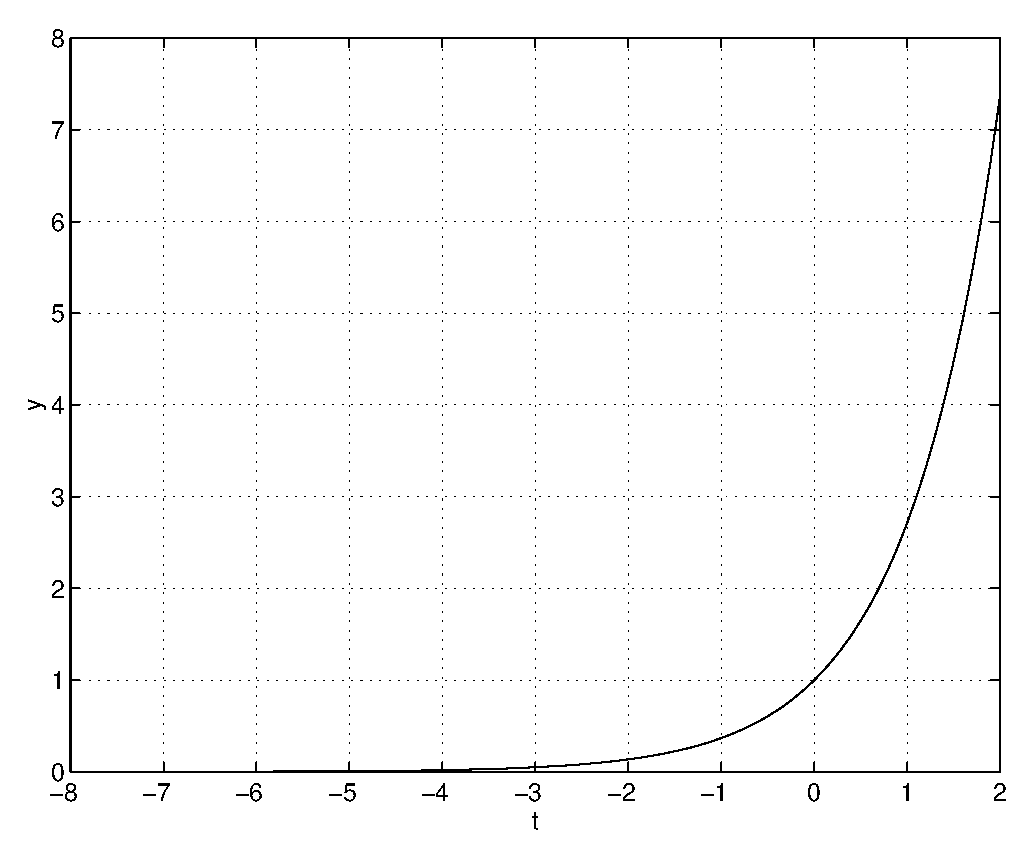
\psfig{file=exfigure/4-4-5a.eps,width=1.8in}
                       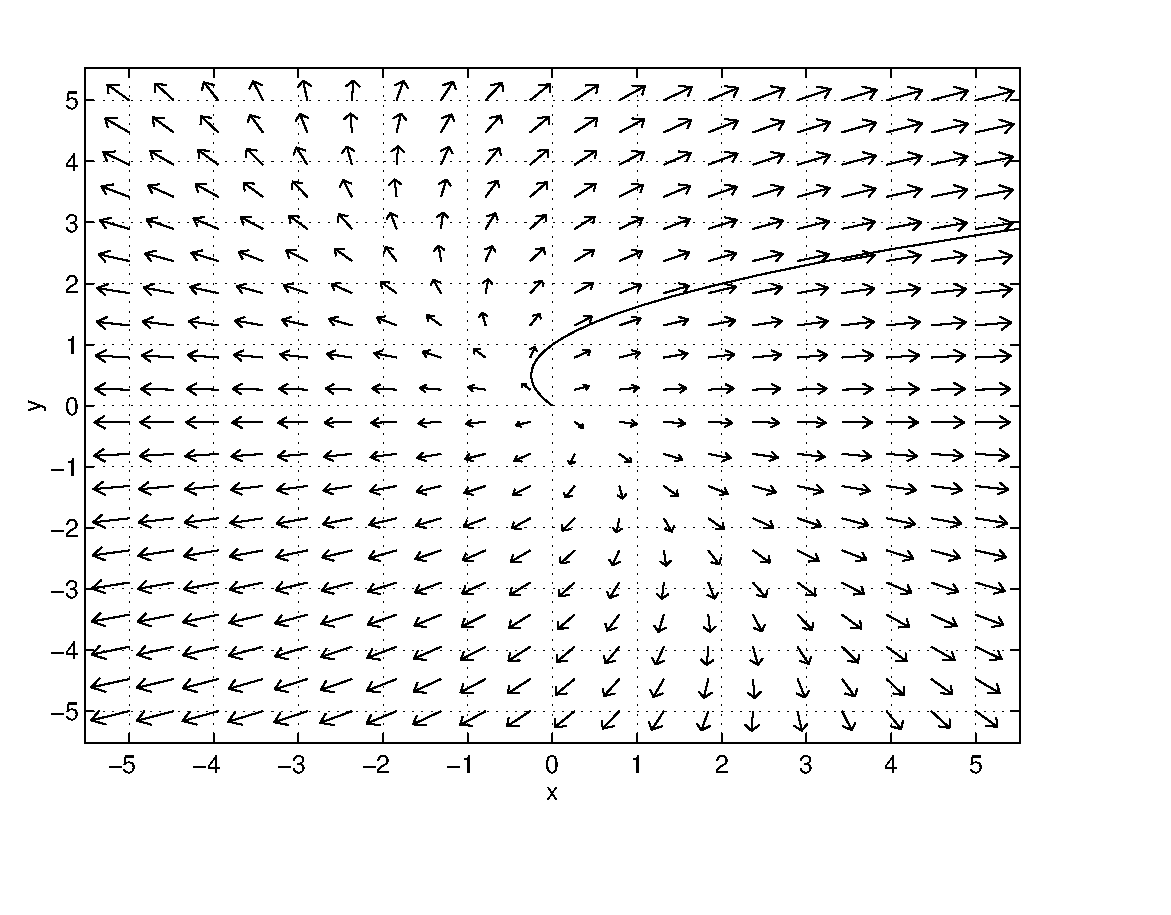
\psfig{file=exfigure/4-4-5b.eps,width=1.8in}
                       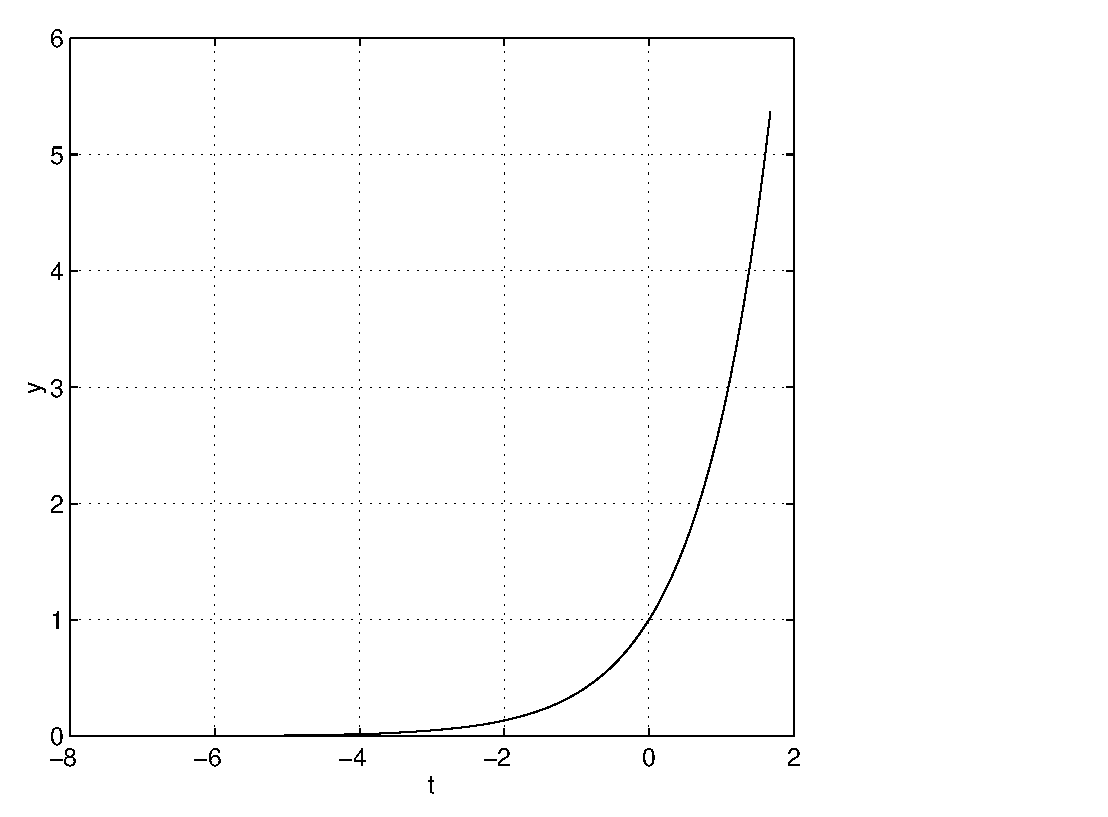
\psfig{file=exfigure/4-4-5c.eps,width=1.8in}}
                \exercapthree{c4.4.5}
\end{figure}






\end{solution}
\end{exercise}


\end{document}

%%% Local Variables:
%%% mode: latex
%%% TeX-master: "../linearAlgebra"
%%% End:
